%!TEX root =  tfg.tex
\chapter{Manual de usuario}

\begin{quotation}[Diseñador e inventor]{Donald A. Norman (1935--)}
Good design is actually a lot harder to notice than poor design, in part because good designs fit our needs so well that the design is invisible.
\end{quotation}

\begin{abstract}
Este capítulo describe la interfaz de Scubex desde el punto de vista del usuario. Se presenta primero cada módulo de la aplicación por separado, y al final se ilustra su uso conjunto mediante tres casos de uso que reflejan perfiles de usuario distintos.
\end{abstract}

% ─────────────────────────────────────────────────────────────────────────────
\section{¿Qué es Scubex?}
\label{sec:manual-que-es}
% ─────────────────────────────────────────────────────────────────────────────

Scubex es una aplicación web para buceadores que reúne en un único lugar tres fuentes de información que habitualmente están separadas: la fauna marina de una zona, las condiciones climáticas y oceanográficas del momento, y las experiencias de otros buceadores.

El punto de partida es siempre un mapa interactivo. El usuario selecciona cualquier punto del océano y puede, sin salir de esa pantalla, consultar qué especies han sido registradas científicamente en los alrededores, comprobar si las condiciones del día son aptas para bucear, y ver qué han publicado otros buceadores en esa misma zona. Si quiere dejar constancia de una inmersión propia, puede publicarla directamente sobre el mapa con una foto y una descripción, y el resto de la comunidad podrá verla, comentarla o guardarla.

Scubex no requiere instalar nada: funciona desde cualquier navegador moderno, en ordenador o en móvil.

% ─────────────────────────────────────────────────────────────────────────────
\section{Autenticación}
\label{sec:manual-auth}
% ─────────────────────────────────────────────────────────────────────────────

Al abrir Scubex por primera vez se muestra la pantalla de inicio (Fig.~\ref{fig:landingPage}). El acceso se realiza mediante una cuenta de Google: basta con pulsar el botón \textit{Iniciar sesión con Google} y seleccionar la cuenta en la ventana emergente del navegador.

\begin{figure}[H]
\begin{center}
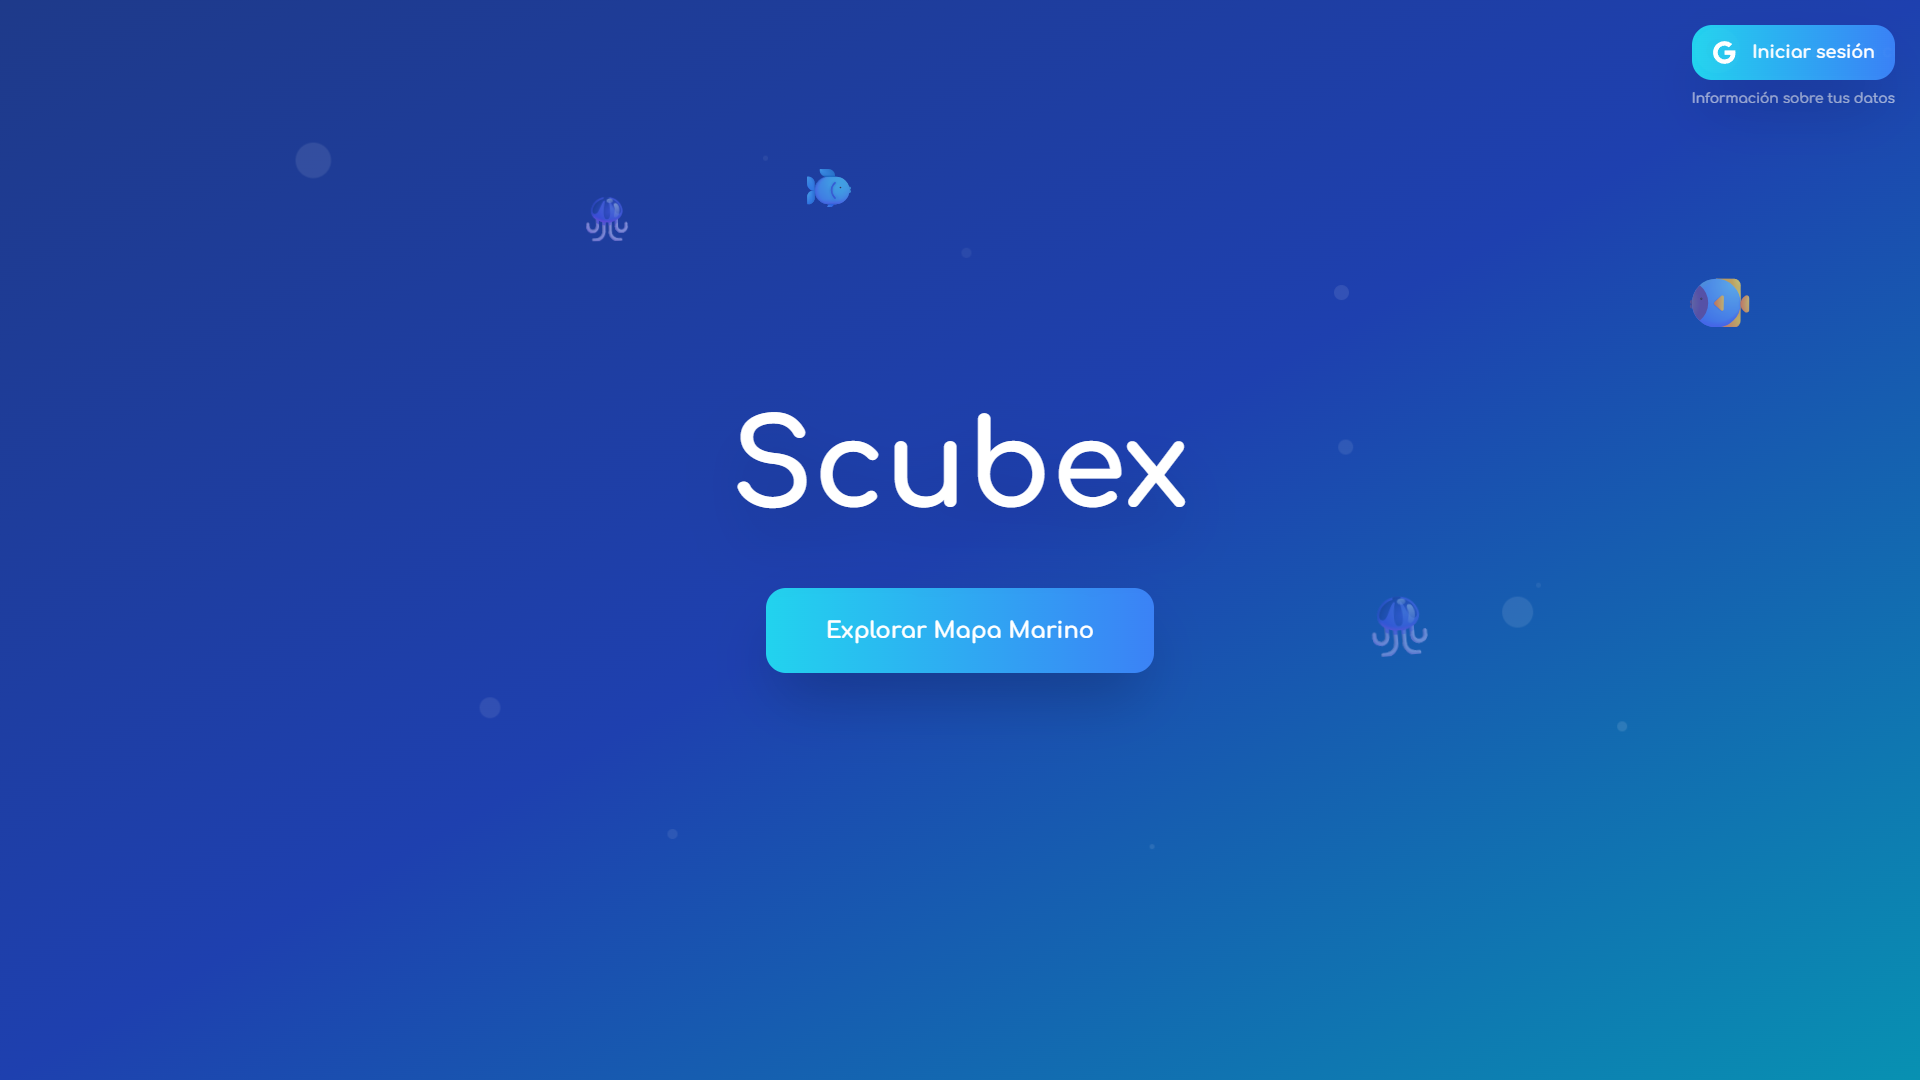
\includegraphics[width=0.75\textwidth]{figures/manual/LandingPage.png}
\caption{Pantalla de inicio de Scubex\label{fig:landingPage}}
\end{center}
\end{figure}

La pantalla no es estática: a medida que el usuario permanece en ella, van apareciendo criaturas marinas que se desplazan a distintas velocidades según la especie, llenando poco a poco la pantalla (Fig.~\ref{fig:landingAnimales}). Cuanto más tiempo se esté en la página, más fauna se acumula.

\begin{figure}[H]
\centering
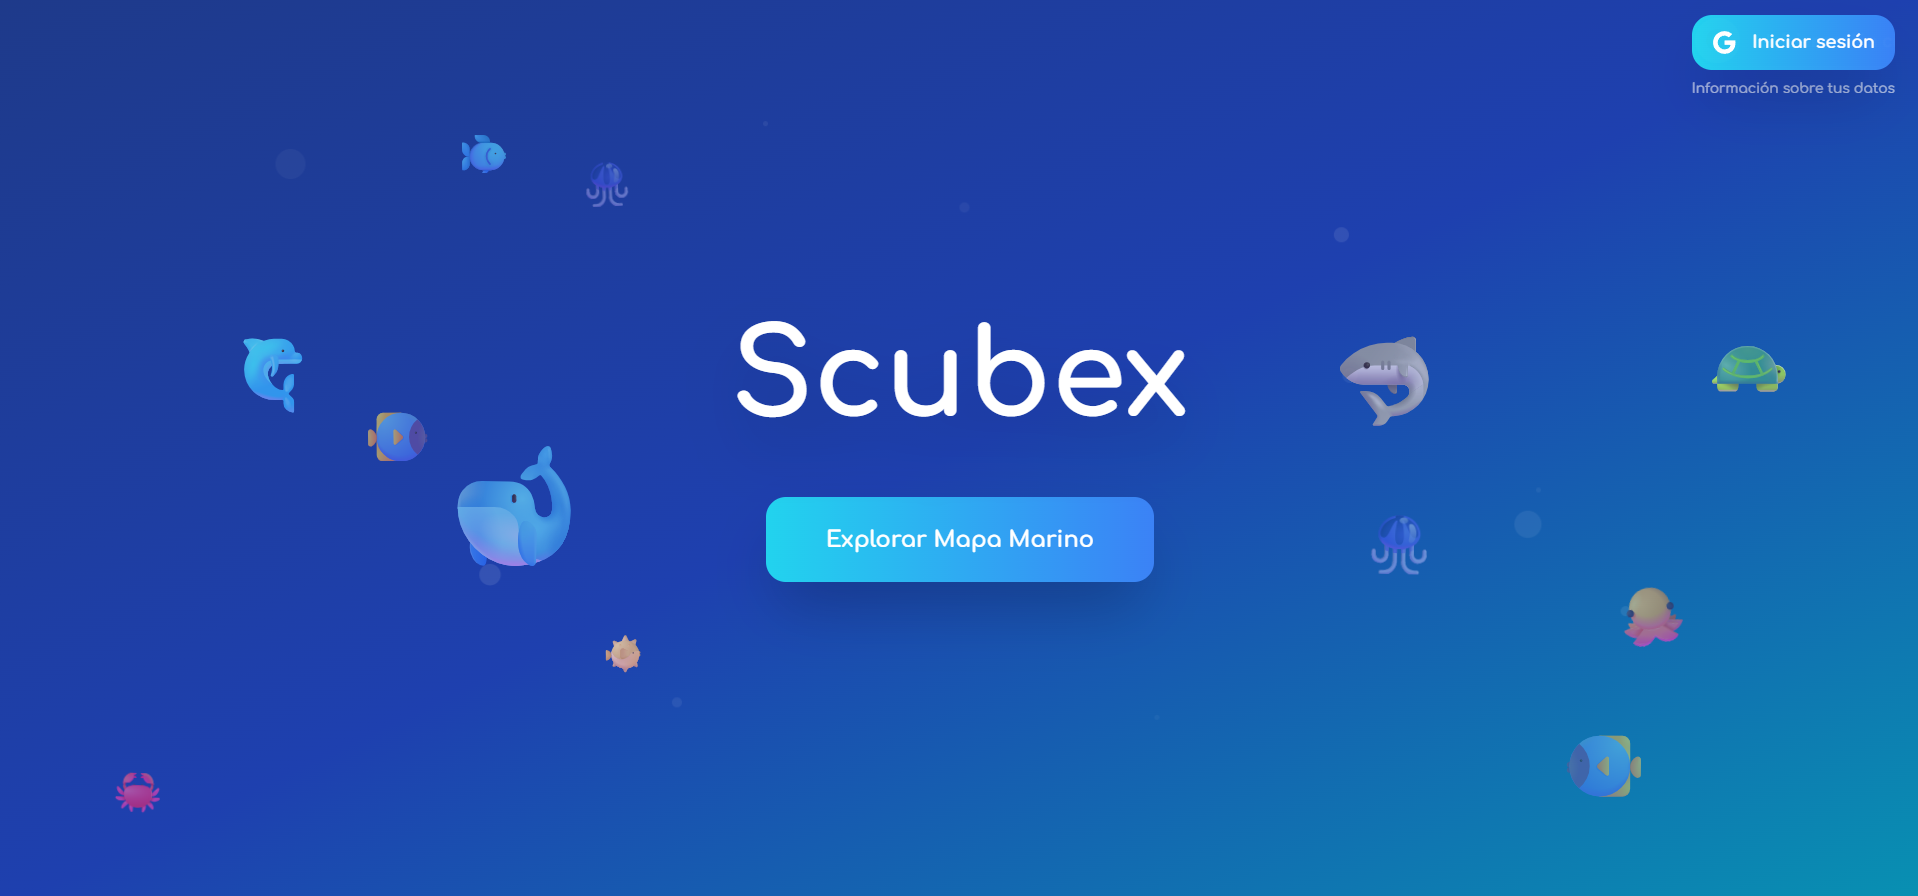
\includegraphics[width=0.85\textwidth]{figures/manual/PaginaInicialConMuchosAnimales.png}
\caption{Pantalla de inicio con la fauna animada acumulada tras unos segundos\label{fig:landingAnimales}}
\end{figure}

Antes de autenticarse, el usuario puede consultar el aviso de privacidad pulsando el enlace correspondiente. Scubex únicamente solicita el nombre, el correo electrónico y la foto de perfil, que se usan exclusivamente para identificar al autor de publicaciones y comentarios (Fig.~\ref{fig:infoDatos}).

\begin{figure}[H]
\begin{center}
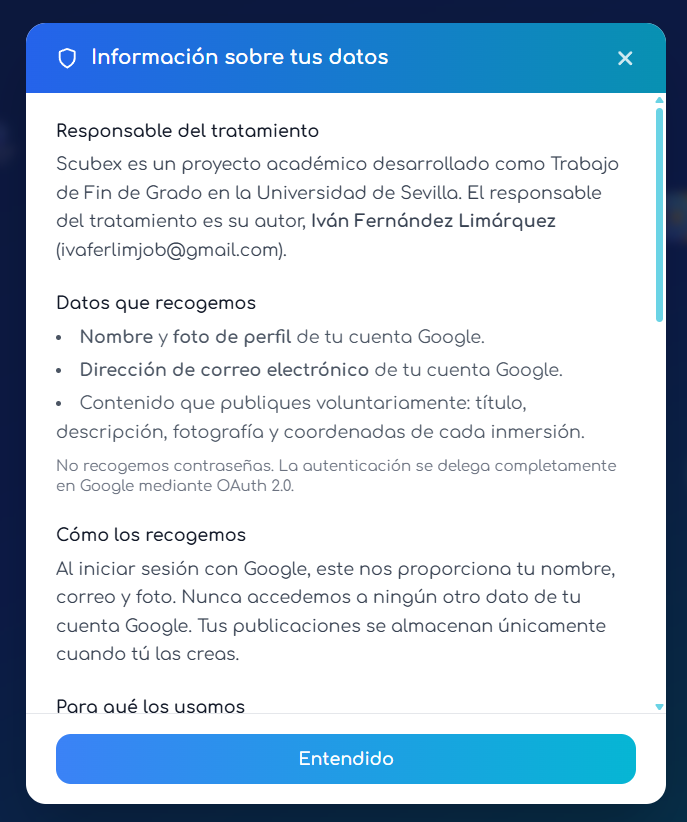
\includegraphics[width=0.55\textwidth]{figures/manual/InfoDeDatos.png}
\caption{Aviso de privacidad y datos recogidos por Scubex\label{fig:infoDatos}}
\end{center}
\end{figure}

Una vez autenticado, el avatar del usuario aparece en la esquina superior derecha de la landing y el botón principal da paso al mapa. La sesión se mantiene activa entre visitas hasta que el usuario la cierra explícitamente desde su perfil.

\begin{figure}[H]
\centering
\begin{minipage}[t]{0.48\textwidth}
  \centering
  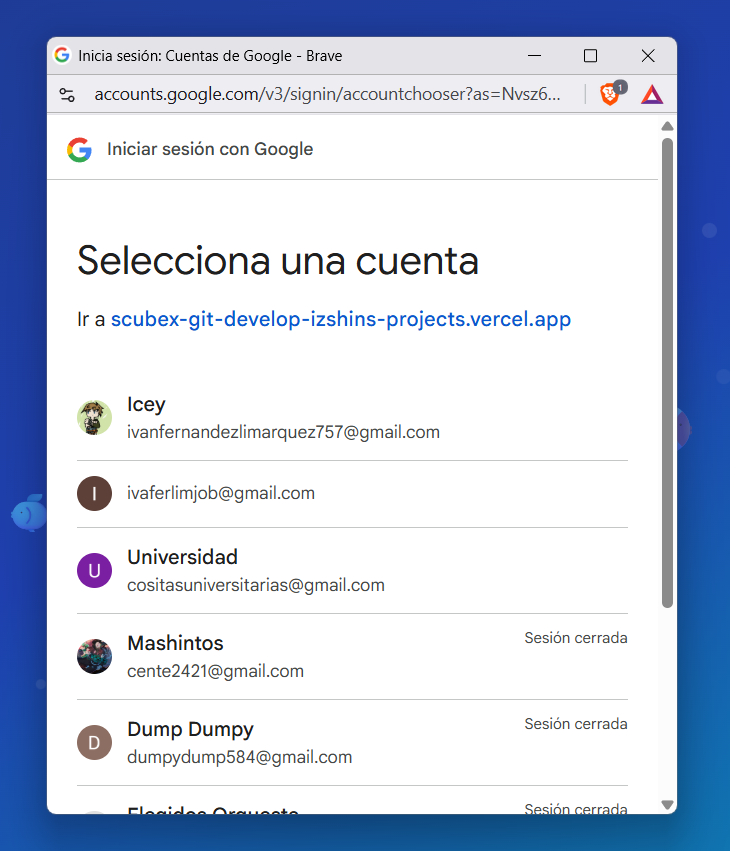
\includegraphics[width=\textwidth]{figures/manual/Autentificación.png}
  \caption{Selector de cuenta de Google\label{fig:autentificacion}}
\end{minipage}
\hfill
\begin{minipage}[t]{0.48\textwidth}
  \centering
  
\includegraphics[width=\textwidth]{figures/manual/avatar.png}
  \caption{Avatar del usuario tras autenticarse\label{fig:avatar}}
\end{minipage}
\end{figure}

% ─────────────────────────────────────────────────────────────────────────────
\section{Exploración del mapa, escaneo, búsqueda y condiciones}
\label{sec:manual-mapa}
% ─────────────────────────────────────────────────────────────────────────────

Al entrar al mapa se muestra una vista oceánica a pantalla completa (Fig.~\ref{fig:mapaGeneral}). En la barra superior aparecen el logotipo de la aplicación a la izquierda, y a la derecha la campana de notificaciones y el avatar del usuario. La lupa en el extremo derecho abre un buscador de lugares: al escribir un nombre de ciudad, bahía o punto de interés, el mapa vuela automáticamente a esa ubicación. En la parte inferior se encuentran los controles principales: el selector de modo (\textit{Escanear} o \textit{Publicar}), el radio de escaneo (2, 5 o 10~km) y el botón para lanzar el escaneo.

\begin{figure}[H]
\centering
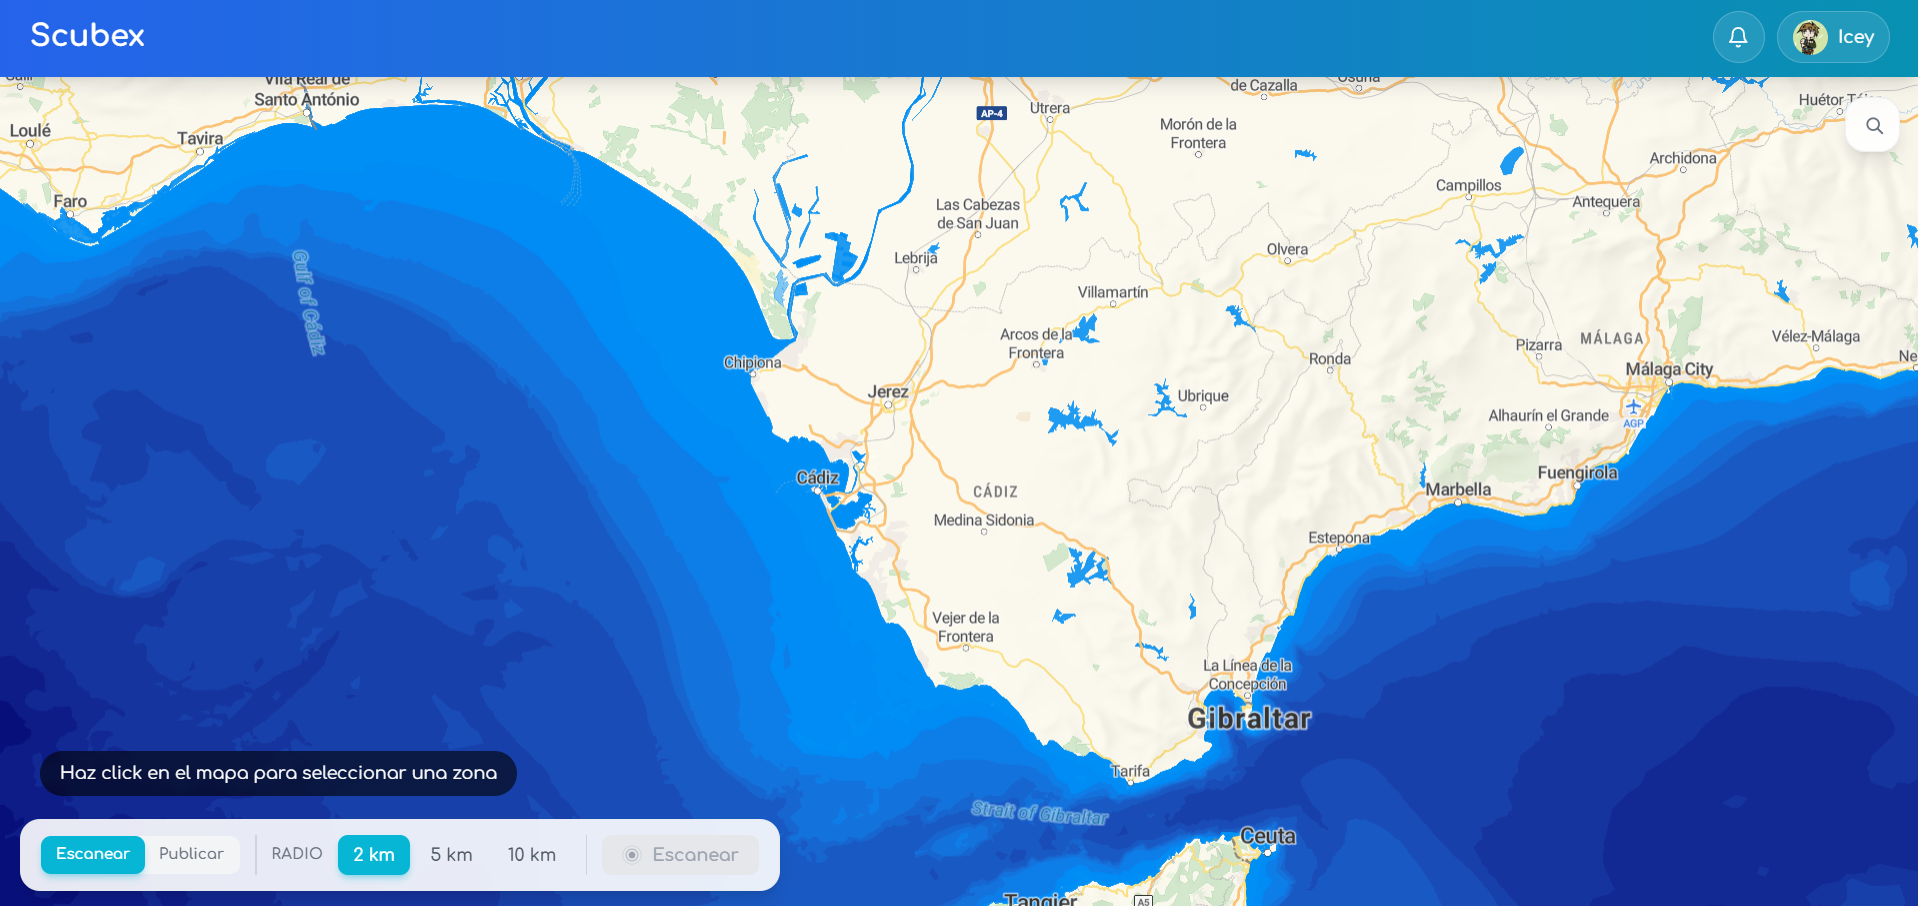
\includegraphics[width=1\textwidth]{figures/manual/MapaGeneral.png}
\caption{Interfaz principal del mapa con los controles de escaneo en la barra inferior\label{fig:mapaGeneral}}
\end{figure}

Para explorar una zona, basta con hacer clic sobre cualquier punto del océano: aparece un marcador y un círculo que delimita el área de búsqueda según el radio seleccionado. Al pulsar \textit{Escanear}, la aplicación consulta las bases de datos científicas OBIS e iNaturalist y obtiene simultáneamente las condiciones climáticas y oceanográficas del punto. Durante la consulta el botón muestra el estado \textit{Escaneando\ldots} y el círculo anima sobre el mapa (Fig.~\ref{fig:modoEscaneo}).

\begin{figure}[H]
\centering
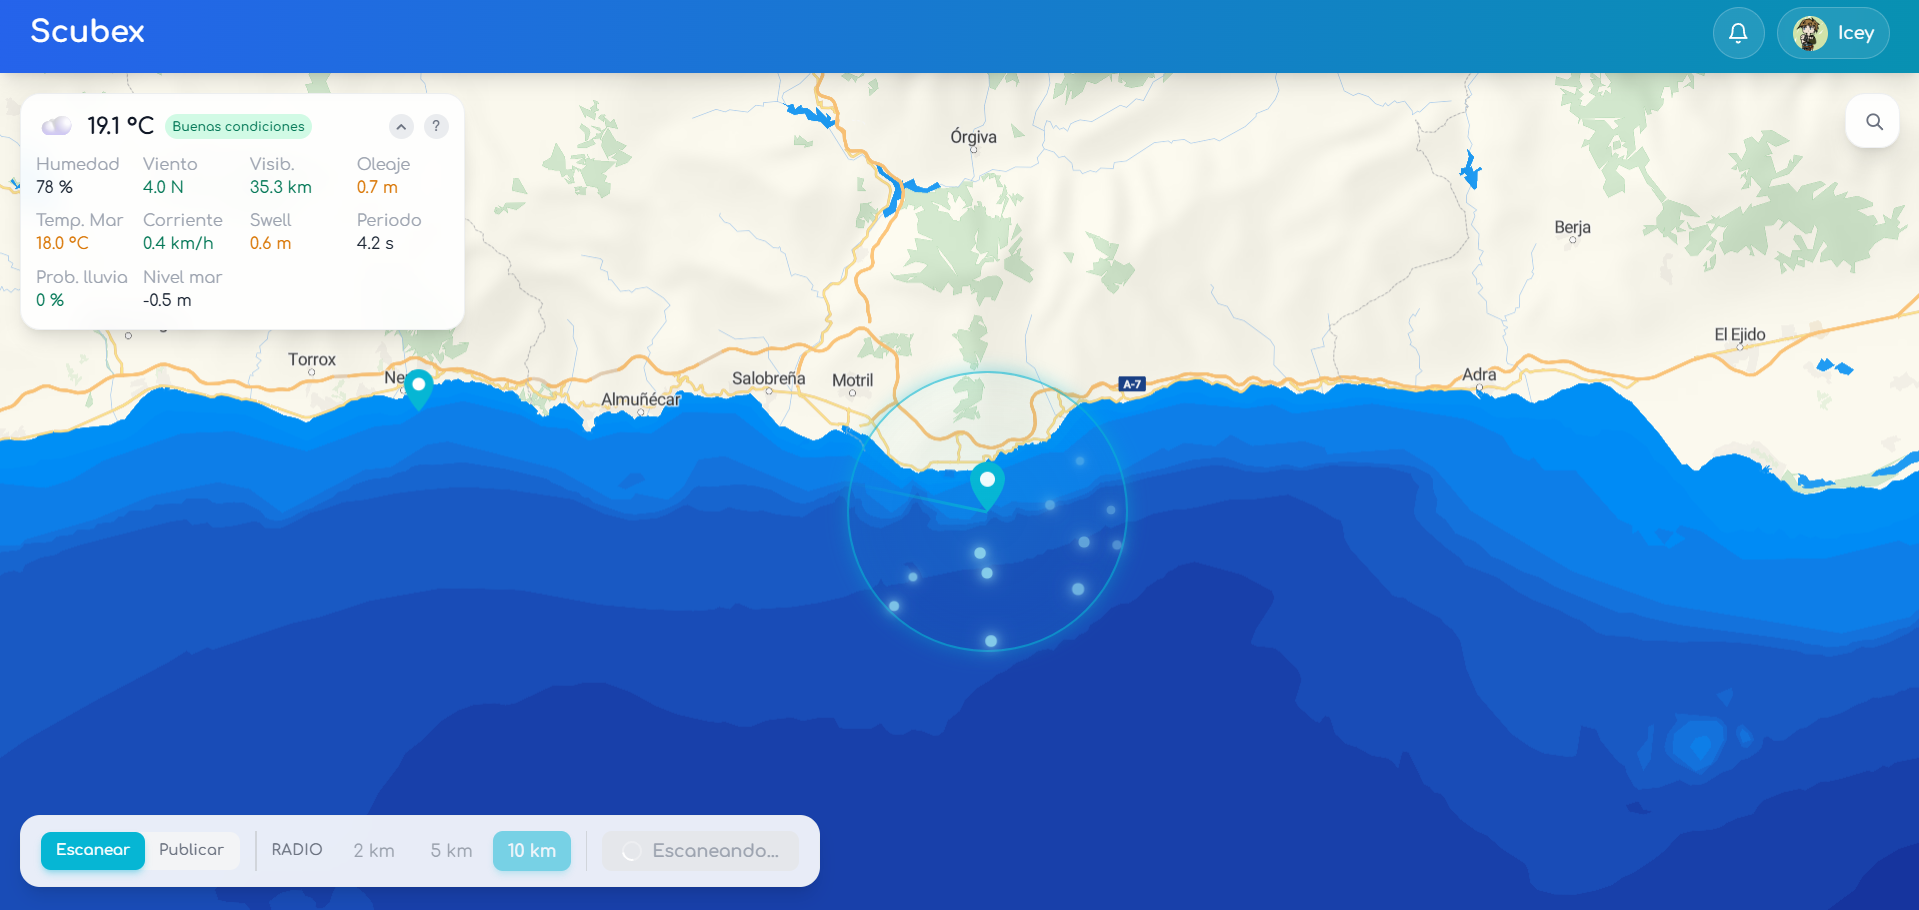
\includegraphics[width=0.85\textwidth]{figures/manual/ModoEscaneo.png}
\caption{Escaneo en curso: círculo de búsqueda sobre el mar y panel climático ya visible\label{fig:modoEscaneo}}
\end{figure}

Al terminar, aparece un aviso en pantalla con el nombre del lugar escaneado (Fig.~\ref{fig:popupEscaneo}). Pulsarlo hace que el mapa vuele hasta el punto y muestre el círculo de búsqueda, útil si el usuario había navegado a otra zona mientras esperaba los resultados.

\begin{figure}[H]
\centering
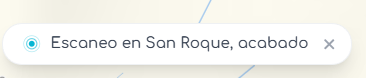
\includegraphics[width=0.55\textwidth]{figures/manual/PopupFinalEscaneo.png}
\caption{Notificación al finalizar el escaneo con el nombre del lugar\label{fig:popupEscaneo}}
\end{figure}

El panel de especies se vuelve entonces desplegable; al abrirlo, el mapa realiza un zoom suave hasta el área escaneada para situar los resultados en contexto (Fig.~\ref{fig:notifPanel}). El panel es colapsable en cualquier momento para recuperar espacio.

\begin{figure}[H]
\centering

\includegraphics[width=0.25\textwidth]{figures/manual/NotificacionAzulPanelEspecies.png}
\caption{Indicador del panel de especies listo para desplegarse\label{fig:notifPanel}}
\end{figure}

\begin{figure}[H]
\centering
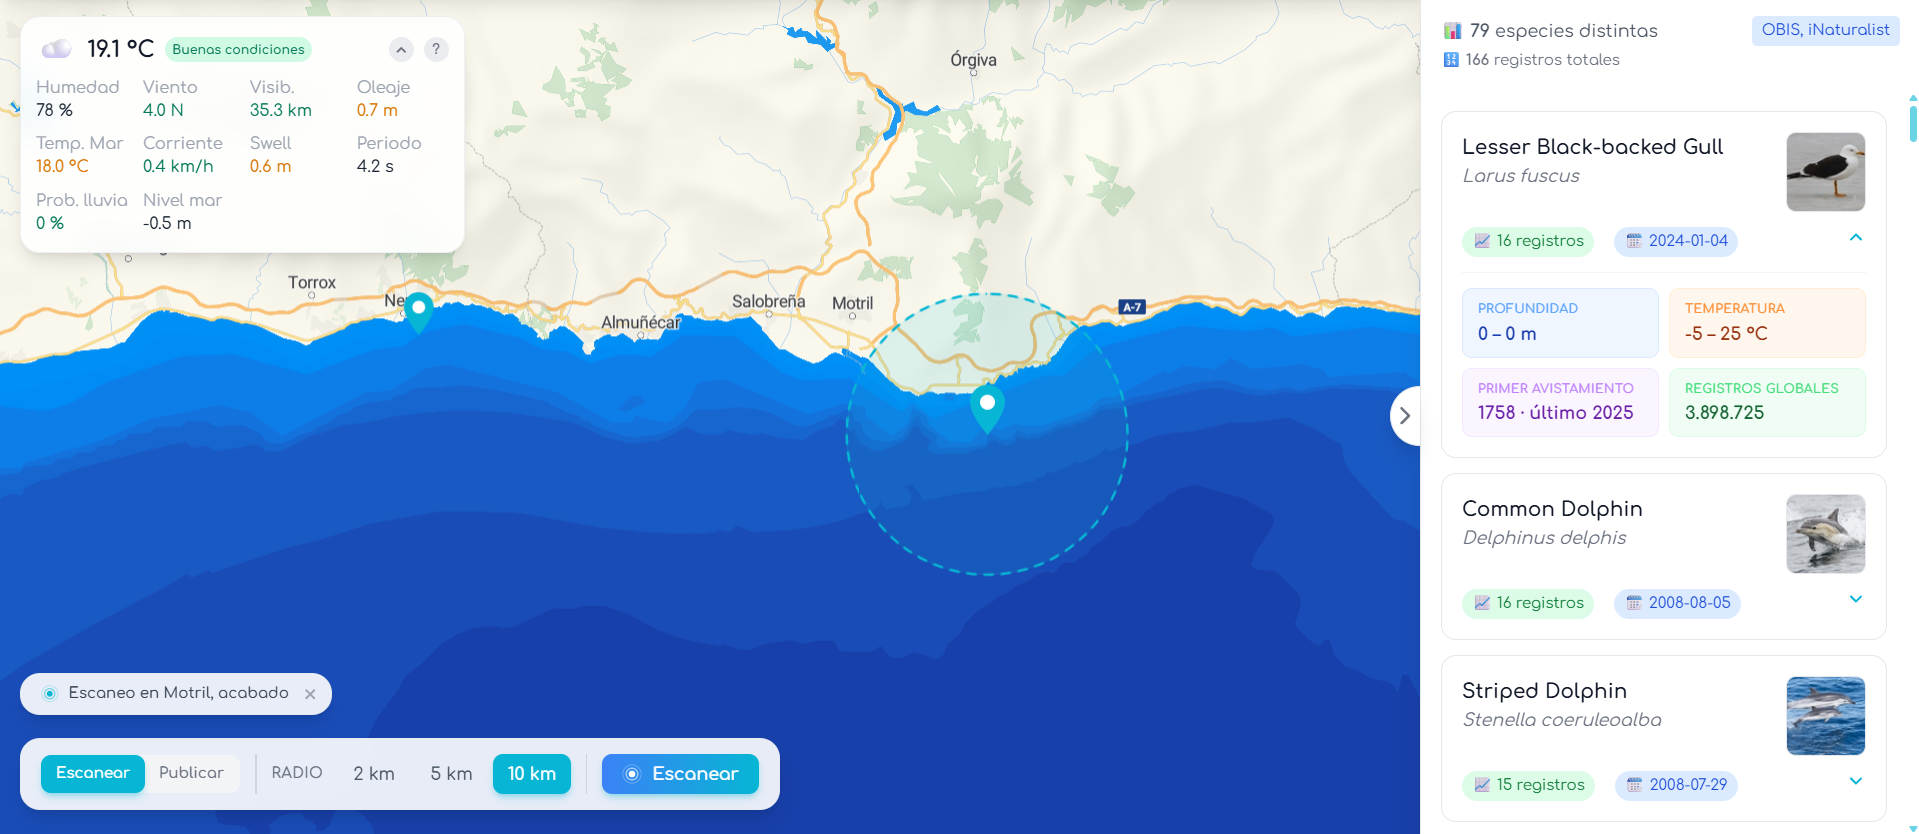
\includegraphics[width=0.85\textwidth]{figures/manual/EscaneoTodoAbierto.png}
\caption{Vista completa con ambos paneles abiertos tras el escaneo\label{fig:escaneoTodoAbierto}}
\end{figure}

El panel de especies lista todas las que han sido registradas en la zona, ordenadas por número de avistamientos. Cada tarjeta muestra el nombre común, el nombre científico y una fotografía de referencia. Al expandirla se accede al rango de profundidad habitual, la temperatura del agua en que se ha observado la especie, la fecha del primer y último registro, y el total de avistamientos globales en la base de datos (Fig.~\ref{fig:panelEspecies}).

\begin{figure}[H]
\centering
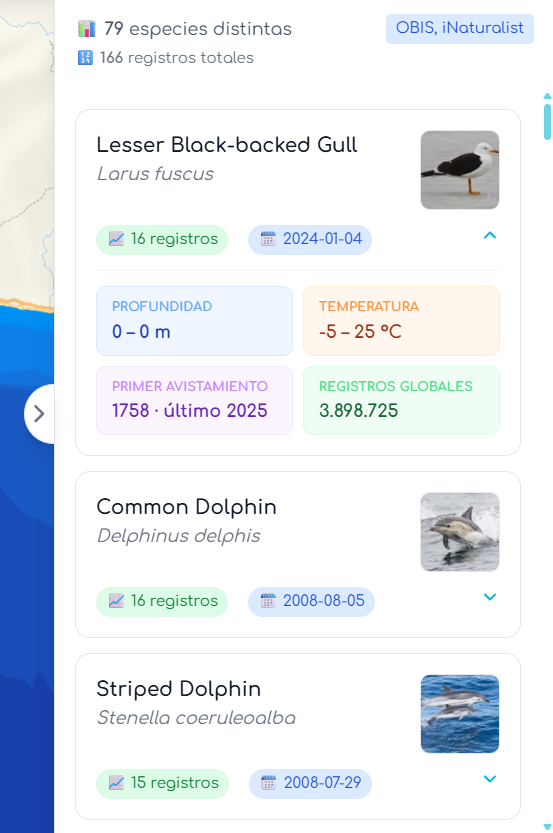
\includegraphics[width=0.5\textwidth]{figures/manual/PanelEspecies.png}
\caption{Panel de especies con una tarjeta expandida mostrando profundidad, temperatura y registros\label{fig:panelEspecies}}
\end{figure}

El panel climático (Fig.~\ref{fig:panelClima}) muestra un resumen compacto en la esquina superior izquierda con la temperatura del aire, un indicador de estado (\textit{Buenas condiciones}, \textit{Condiciones tolerables} o \textit{Condiciones adversas}) y las métricas más relevantes para el buceo: oleaje, corriente, temperatura del mar, visibilidad, viento, swell y probabilidad de lluvia. Pulsando el icono de información se abre un modal con la descripción detallada de cada parámetro y los umbrales que determinan su color (Fig.~\ref{fig:datosClima}).

\begin{figure}[H]
\centering
\begin{minipage}[t]{0.42\textwidth}
  \centering
  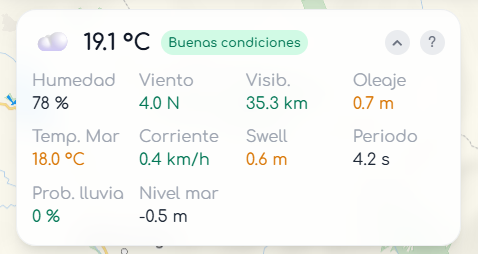
\includegraphics[width=\textwidth]{figures/manual/PanelClima.png}
  \caption{Resumen compacto de condiciones climáticas\label{fig:panelClima}}
\end{minipage}
\hfill
\begin{minipage}[t]{0.54\textwidth}
  \centering
  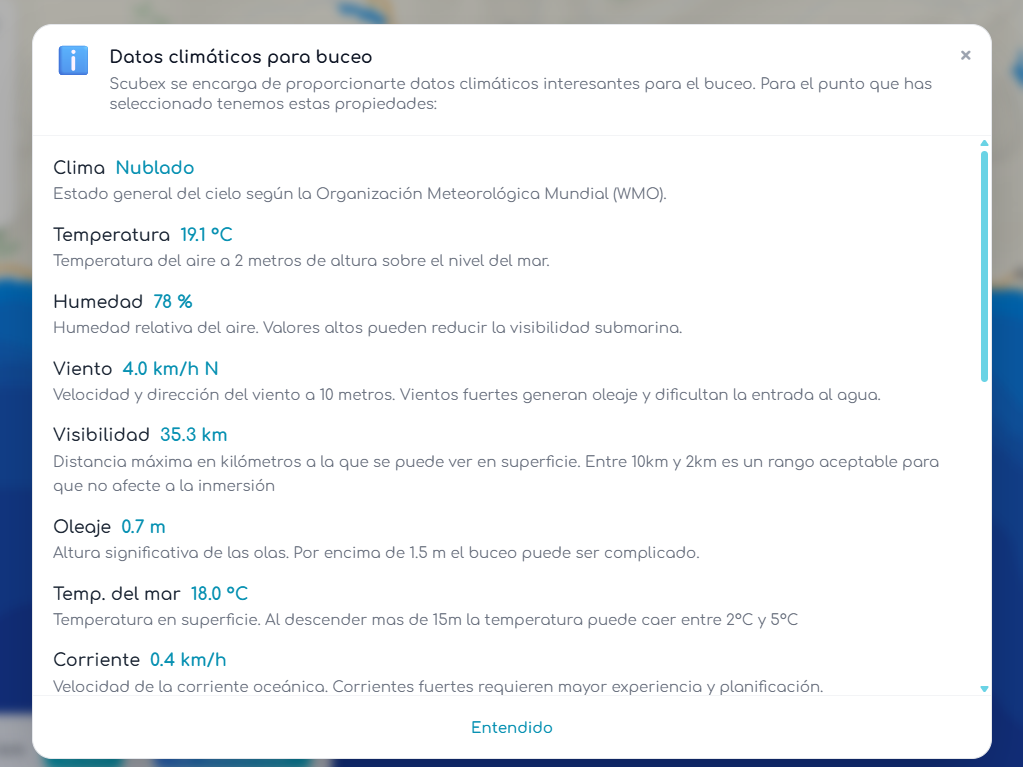
\includegraphics[width=\textwidth]{figures/manual/DatosClima.png}
  \caption{Modal de detalle con la descripción de cada métrica\label{fig:datosClima}}
\end{minipage}
\end{figure}

% ─────────────────────────────────────────────────────────────────────────────
\section{Sistema de publicaciones}
\label{sec:manual-publicaciones}
% ─────────────────────────────────────────────────────────────────────────────

Las publicaciones son el registro de inmersiones de la comunidad. En el mapa aparecen como marcadores celestes repartidos por la costa (Fig.~\ref{fig:muchasPublicaciones}); su distribución permite hacerse una idea rápida de qué zonas tienen más actividad.

\begin{figure}[H]
\centering
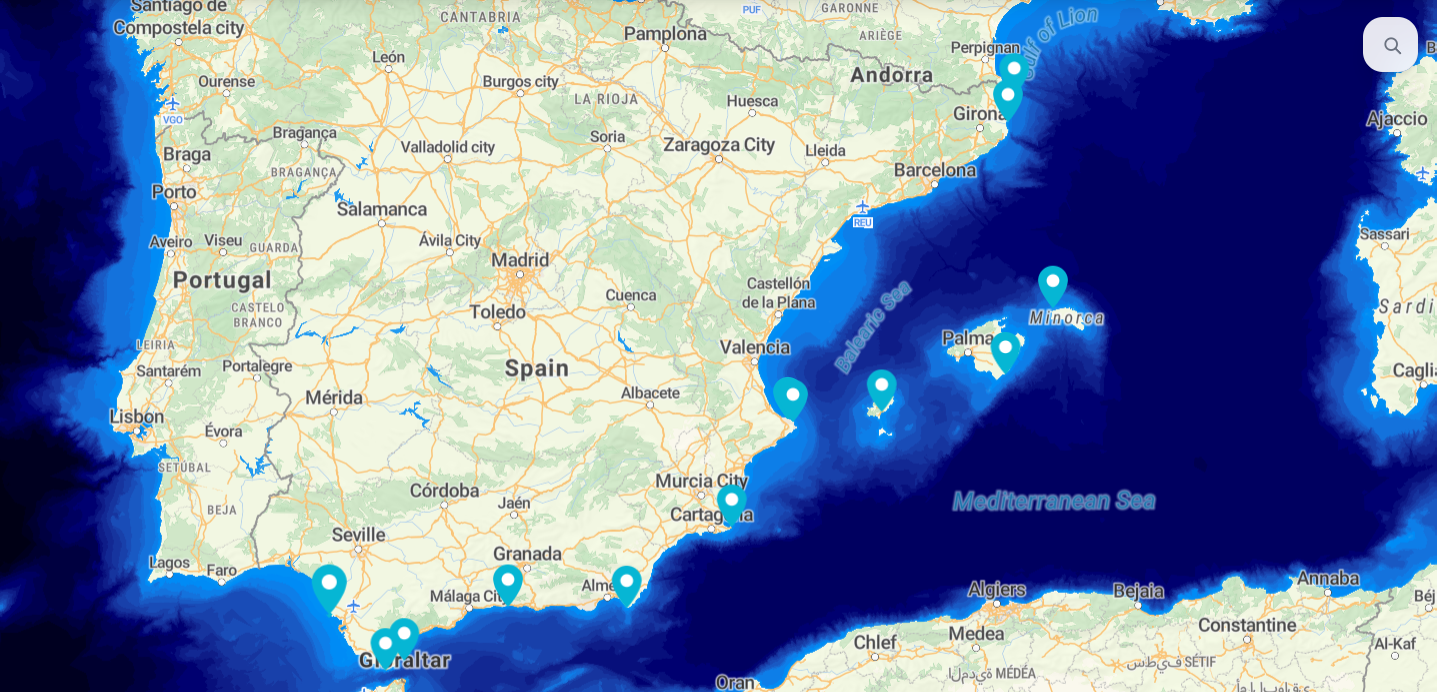
\includegraphics[width=0.85\textwidth]{figures/manual/MuchasPublicacionesMapa.png}
\caption{Marcadores de publicaciones distribuidos por el litoral\label{fig:muchasPublicaciones}}
\end{figure}

Para crear una, hay que cambiar al modo \textit{Publicar} en la barra inferior (Fig.~\ref{fig:modoPublicacion}) y hacer clic sobre el punto del mapa donde se realizó la inmersión.

\begin{figure}[H]
\centering
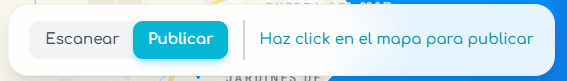
\includegraphics[width=0.7\textwidth]{figures/manual/ModoPublicacion.png}
\caption{Barra inferior en modo Publicar\label{fig:modoPublicacion}}
\end{figure}

Se abre un formulario con título, descripción opcional, el nombre del lugar detectado automáticamente a partir de las coordenadas, y la posibilidad de adjuntar una foto (Fig.~\ref{fig:formularioVacio}). Al añadir una imagen el mapa se desplaza hacia arriba para que el formulario completo quede visible sin que la foto quede cortada (Fig.~\ref{fig:formularioRelleno}).

\begin{figure}[H]
\centering
\begin{minipage}[t]{0.44\textwidth}
  \centering
  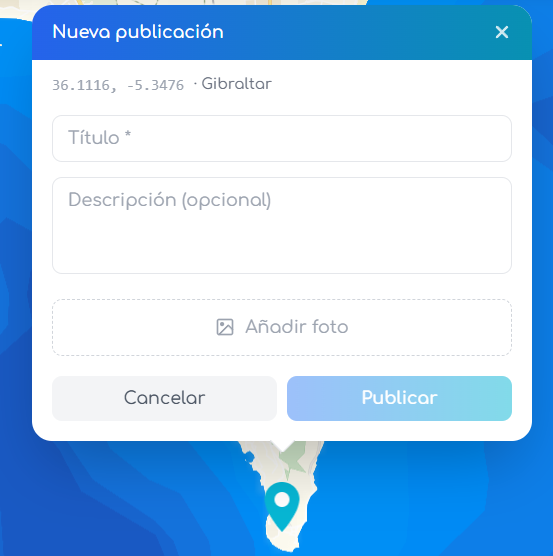
\includegraphics[width=\textwidth]{figures/manual/FormularioPublicacion.png}
  \caption{Formulario de nueva publicación vacío\label{fig:formularioVacio}}
\end{minipage}
\hfill
\begin{minipage}[t]{0.44\textwidth}
  \centering
  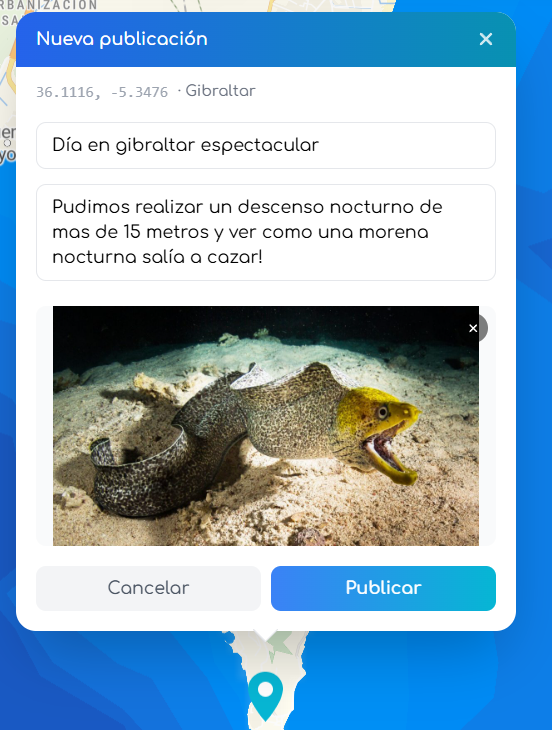
\includegraphics[width=\textwidth]{figures/manual/FormularioPublicaciónRelleno.png}
  \caption{Formulario con título, descripción y foto cargada\label{fig:formularioRelleno}}
\end{minipage}
\end{figure}

Al publicar, el marcador aparece en el mapa y al pulsarlo se abre una tarjeta con el título, la descripción, la imagen y el enlace \textit{Ver más} para expandir el detalle completo (Fig.~\ref{fig:publicacionCreada}).

\begin{figure}[H]
\centering
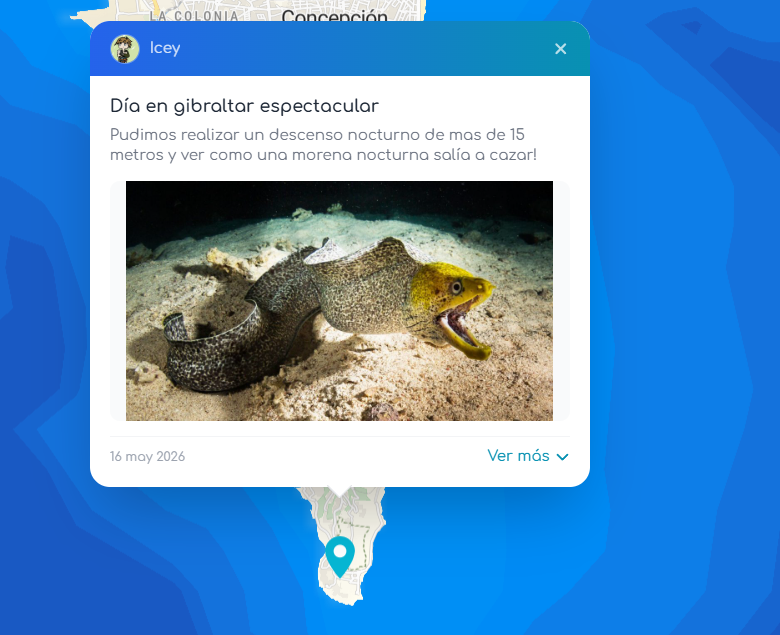
\includegraphics[width=0.6\textwidth]{figures/manual/PublicacionRecienCreada.png}
\caption{Tarjeta compacta de una publicación recién creada\label{fig:publicacionCreada}}
\end{figure}

El panel de detalle completo muestra el autor con su nombre, la fecha, el título, la descripción, la foto y el nombre del lugar correspondiente al punto marcado en el mapa (Fig.~\ref{fig:detallesPublicacion}). En la parte inferior aparecen los controles de interacción: like, comentarios, compartir y guardar.

\begin{figure}[H]
\centering
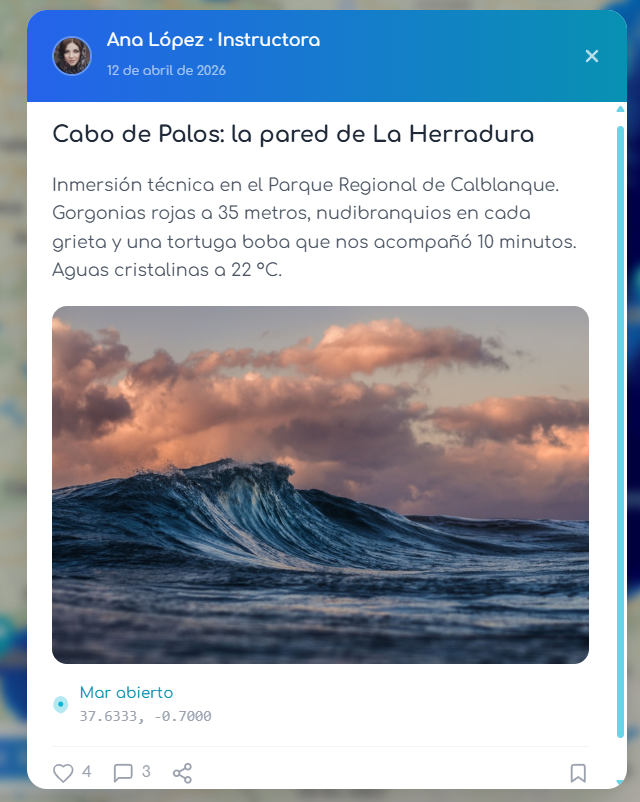
\includegraphics[width=0.55\textwidth]{figures/manual/DetallesPublicacion.png}
\caption{Panel de detalle completo de una publicación\label{fig:detallesPublicacion}}
\end{figure}

El like se activa con un toque y actualiza el contador de forma inmediata. Los comentarios se despliegan debajo y el panel hace un pequeño desplazamiento automático para dejarlos a la vista; para responder a alguien basta con pulsar el botón \textit{Responder} bajo cualquier comentario, que rellena automáticamente la mención en el campo de texto. El botón de guardar marca la publicación para recuperarla desde el perfil propio. En la Fig.~\ref{fig:interacciones} se ven los tres en uso simultáneo: like dado, sección de comentarios abierta y publicación guardada.

\begin{figure}[H]
\centering
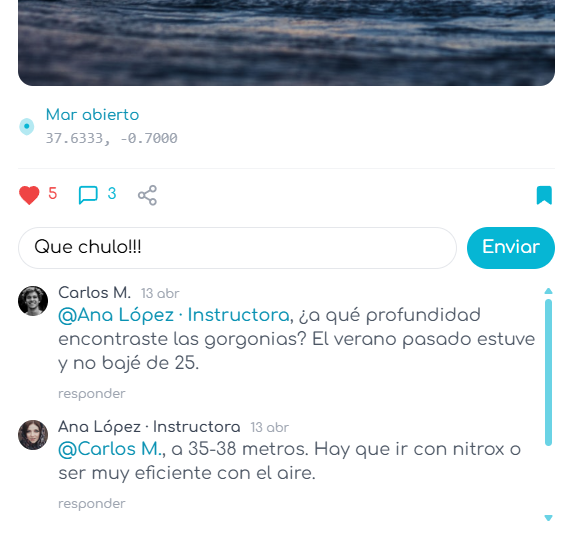
\includegraphics[width=0.55\textwidth]{figures/manual/DetallesPublicacionInteraccionLikeGuardadoComentando.png}
\caption{Like activo, comentarios con mención y publicación guardada\label{fig:interacciones}}
\end{figure}

Todas estas interacciones generan notificaciones para el autor de la publicación. Cómo consultarlas y el resto de la capa social se describe en la siguiente sección.

% ─────────────────────────────────────────────────────────────────────────────
\section{Red social}
\label{sec:manual-social}
% ─────────────────────────────────────────────────────────────────────────────

% TODO: Perfil propio: editar nombre y foto, pestañas Publicaciones/Guardados, estadísticas de seguidores/seguidos.
% TODO: Perfil ajeno: follow/unfollow, ver sus publicaciones, compartir perfil.
% TODO: Listas de seguidores y seguidos: modal, navegar a perfiles desde la lista.
% TODO: Guardados: cómo guardar una publicación y acceder a la colección desde el perfil.

% ─────────────────────────────────────────────────────────────────────────────
\section{Consideraciones estéticas y de flujo}
\label{sec:manual-estetica}
% ─────────────────────────────────────────────────────────────────────────────

\subsection{Estética e interfaz}
\label{sec:manual-ui}

Scubex mantiene un lenguaje visual coherente a lo largo de toda la interfaz. Los elementos interactivos o activos se identifican siempre por el mismo color celeste: el modo seleccionado en la barra inferior, el radio de escaneo activo, los botones de acción principal o cualquier opción marcada en un selector aparecen en ese tono (Fig.~\ref{fig:patronCeleste}). La única excepción deliberada es el like, que sigue el rojo del corazón ya establecido por otras redes sociales, aprovechando un patrón que el usuario reconoce sin necesidad de aprenderlo.

\begin{figure}[H]
\centering
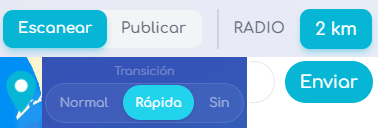
\includegraphics[width=0.6\textwidth]{figures/manual/PatronColorCeleste.png}
\caption{Color celeste como indicador de elemento activo o acción disponible\label{fig:patronCeleste}}
\end{figure}

\subsection{Flujo y experiencia}
\label{sec:manual-ux}

Las transiciones entre pantallas se realizan mediante una animación de ola que recorre la pantalla de lado a lado. Su velocidad es configurable desde el perfil del usuario: la opción rápida reduce la duración al mínimo para quienes prefieren una navegación más directa.

Las acciones que dependen del servidor, como el like o el guardado, se reflejan en la interfaz antes de que llegue la confirmación: el contador sube y el icono cambia de estado al instante, sin esperar la respuesta. Si algo falla, la interfaz revierte el cambio de forma silenciosa. El resultado es que la aplicación se siente rápida incluso con conexiones lentas.
